\chapter{{\bf Summary and Outlook}}
\label{sec:summaryandoutlook}

\section{Summary}
The LHCb experiment was built to test the predictions of the SM and search for NP effects through the study of $\mathcal{CP}$ violating and rare decays of $b$-hadrons. So far measurements performed using the LHCb experiment, and other LHC experiments, have not revealed conclusive evidence for NP effects, although some interesting anomalies have been seen in measured results in heavy flavour physics~\cite{PhysRevLett.118.111801,Aaij:2014pli, Aaij:2015oid. ATLAS-CONF-2017-023,CMS-PAS-BPH-15-008,Aaij:2015esa,PhysRevLett.113.151601,R_K_star,Aaij:2015yra,Huschle:2015rga, Lees:2012xj,Lees:2013uzd, Sato:2016svk,Altmannshofer:2017yso,Capdevila:2017bsm,Amhis:2016xyh}. 
%~\cite{PhysRevLett.118.111801,Aaij:2014pli,Aaij:2015yra,Lees:2013uzd,Huschle:2015rga,Lees:2012xj,Aaij:2015oid,Aaij:2015esa,PhysRevLett.113.151601, R_K_star}. %show no significant deviations from predictions and confirm the predictive power of the SM. 
The search for \bmumu decays was identified as one of the key measurements to be made with the LHCb experiment~\cite{Adeva:2009ny} as an indirect search for NP.
In 2011 LHCb joined the search for these decays, that began over 30 years ago, using the unprecedented energies available at the LHC. The first evidence for \bsmumu decays was found by the LHCb experiment with 2.1 \fb of Run~1 data from $pp$ collisions~\cite{Aaij:2012nna}. A combined analysis of the Run~1 data from the CMS and LHCb experiments produced the first observation of \bsmumu decays and the first evidence for \bdmumu decays~\cite{CMS:2014xfa}. The measured branching fractions of these decays are consistent with the SM predictions and place constraints on BSM theories, However, the precision of the measurements still leaves room for NP effects to be revealed, therefore it is important to improve the precision of the \BF measurements. With the observation of the \bs mode the search for \bsmumu decays is complete and properties of this decays, including the effective lifetime, can now be studied. The effective lifetime offers a new observable to test the SM in \bsmumu decays that is complementary to the \BF. 

The measurements of the \bmumu \BFs and the \bsmumu effective lifetime with 4.4~\fb of Run~1 and Run~2 data collected by the LHCb experiment are presented in this dissertation. The measured \BFs are
\begin{equation}
%\begin{align}                                                                            
\begin{split}
  \mathcal{B}(B^{0}_{s} \to \mu^{+} \mu^{-}) &= (3.0 \pm 0.6^{+0.3}_{-0.2}) \times 10^{-9\
} \\
  \mathcal{B}(B^{0} \to \mu^{+} \mu^{-}) &= (1.5^{+1.2 +0.2}_{-1.0 -0.1})    \times 10^{-\
10}.
%\end{align}                                                                              
\end{split}
\label{eq:BFresults2}
\end{equation}
The \bs mode is observed with a statistical significance of 7.8$\sigma$, making this result the first single experiment observation of this decay and the most precise measurement to date. The \bd mode is observed with a significance of 1.6$\sigma$, therefore a limit is placed on the \BF of $\mathcal{B}$(\bdmumu)$ < 3.4 \times 10^{-10}$ at the 95$\%$ confidence level. The measured values are consistent with the SM predictions and Figure~\ref{fig:BDT} shows \bmumu candidates with a global BDT value of BDT > 0.5. %plot of Bd bv Bs?? with the others superimposed?
\begin{figure}[tbp]
    \centering
        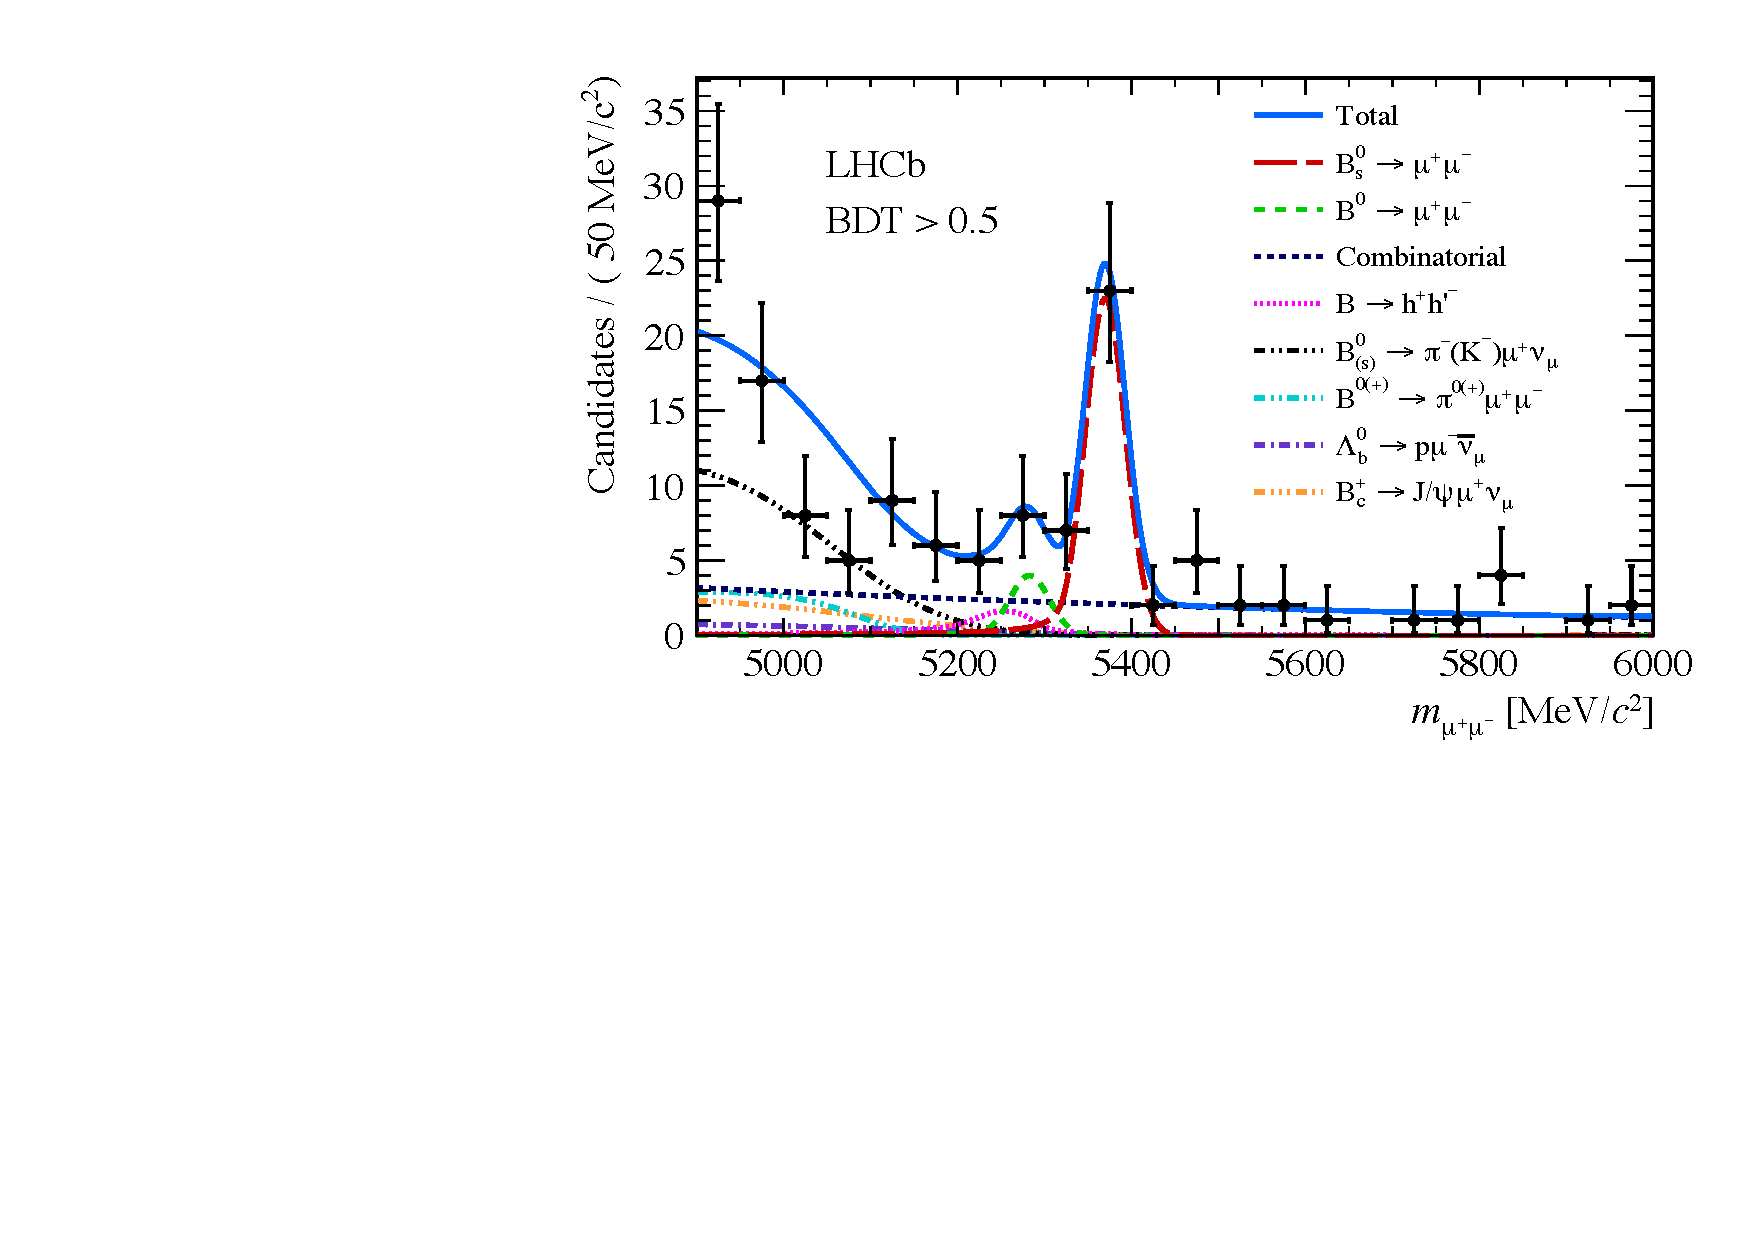
\includegraphics[width=0.8\textwidth]{./Figs/Summary/BDT_plot.pdf}
    \caption{\bmumu candidates with a global BDT value of BDT > 0.5 and the mass fit used to measure the \bmumu \BFs overlaid.}
    \label{fig:BDT}
\end{figure}

The effective lifetime of \bsmumu decays is measured for the first time to be 
\begin{equation}
\tau_{\mu\mu} = 2.04 \pm 0.44 \pm 0.05 \text{ ps},
\end{equation}
which is within 1.0$\sigma$ of the SM prediction. The result is consistent with \ADG = +1 hypothesis at 1.0$\sigma$ and with \ADG = $-1$ hypothesis at 1.4$\sigma$. Although the current precision of the measurement does not enable constraints to be placed on BSM theories it is important to illustrate the ability of the LHCb experiment to make this measurement.

The measured values of the \BF presented in this dissertation have already been used to help constrain parameters in BSM theories~\cite{Altmannshofer:2017wqy,Fleischer:2017ltw,Bobeth:2017xry,Chiang:2017etj}. 
The possible values available for the parameters $P$ and $S$, defined in Section~\ref{sec:BFdef}, are shown in Figure~\ref{fig:NPcontss}, where the values are constrained from the \BF results in Equation~\ref{eq:BFresults2} and the results from the CMS collaboration in reference~\cite{Chatrchyan:2013bka}. The current measurements produce a circular band of possible $P$ and $S$ values, and a precise measurement of \ADG through the \bsmumu \el will help resolve the ambiguities.


\begin{figure}[tbp]
    \centering
        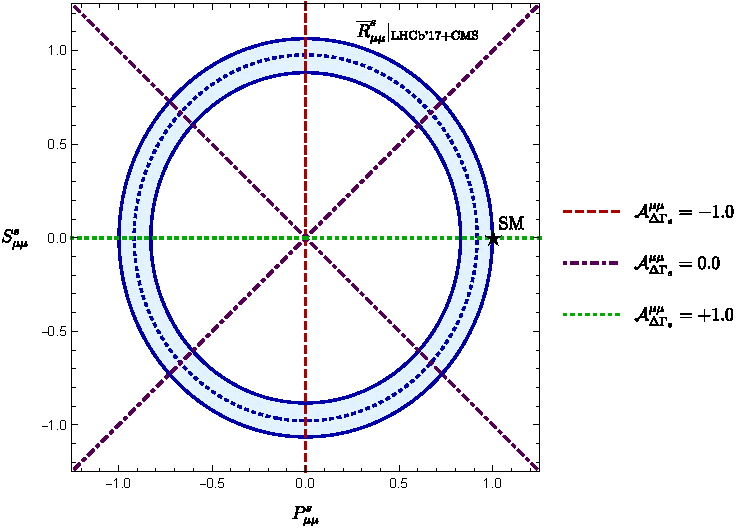
\includegraphics[width=0.7\textwidth]{./Figs/Summary/fig3.pdf}
    \caption{Constraints in the $P$ - $S$ plane where $P$ and $S$ are defined in Section~\ref{sec:BFdef}. The blue band corresponds to constraints from the \bmumu \BF measurements presented in this dissertation and the CMS collaboration results in reference~\cite{Chatrchyan:2013bka} and the dashed lines show different values for \ADG. The constraints assume $\varphi_{P}, \varphi_{S}\in {0, \pi}$. The figure is taken from~\cite{Fleischer:2017ltw}.}
    \label{fig:NPcontss}
\end{figure}


\section{Outlook}
The measured values of the branching fractions and the effective lifetime still leave plenty of room for NP effects to be observed with these decays. At the end of Run~2 of the LHC, the LHCb dataset will have almost doubled to 8~\fb, enabling the precision of these measurements to be improved. Looking further ahead, LHCb is expected to collect 50~\fb of data by the end of Run~4 and with the high luminosity LHC up to 300~\fb could be recorded. 

With more data, the expected precision of the \BF measurements is expected to be reduced to $\sim 0.19 \times 10^{-9}$ with 50~\fb~\cite{LHCb-PUB-2014-040}. Not only are the \BF measurements in themselves interesting to test the SM but the ratio of the \BFs of the two modes is also useful to test the SM, in particular the MFV hypothesis. The current precision of the ratio of \BFs is $\sim 60\%$~\cite{CMS:2014xfa}, the future runs of the LHC will enable the precision of the ratio of \BFs to be reduced to 40$\%$ with 50~\fb of $pp$ data and 20$\%$ with 300~\fb of data~\cite{Aaij:2244311}. 

The expected uncertainty achievable by the LHCb experiment for the \el at the end of Run~2 and after future runs of the LHC is estimated using pseudoexperiments based on the observed numbers of decays with 4.4~\fb and the current measurement strategy. At the end of Run~2, with 8~\fb, the median uncertainty of the \el will be $\sim$0.2 \ps which is reduced to $\sim$0.08~\ps with 50~\fb and $\sim$0.03~\ps with 300~\fb. Therefore, with 300~\fb the precision on the effective lifetime will be able to distinguish NP effects. The expected mass and decay time distributions for 8, 50 and 300~\fb are shown in Figure~\ref{fig:expected_dist}. The expected uncertainties for the \el measurement are conservative estimates because they are based on the current measurement strategy which was designed for low expected statistics. Therefore the precision of the measurement could be much better as different analysis methods can be taken advantage of with more statistics. 


\begin{figure}[tbp]
    \centering
        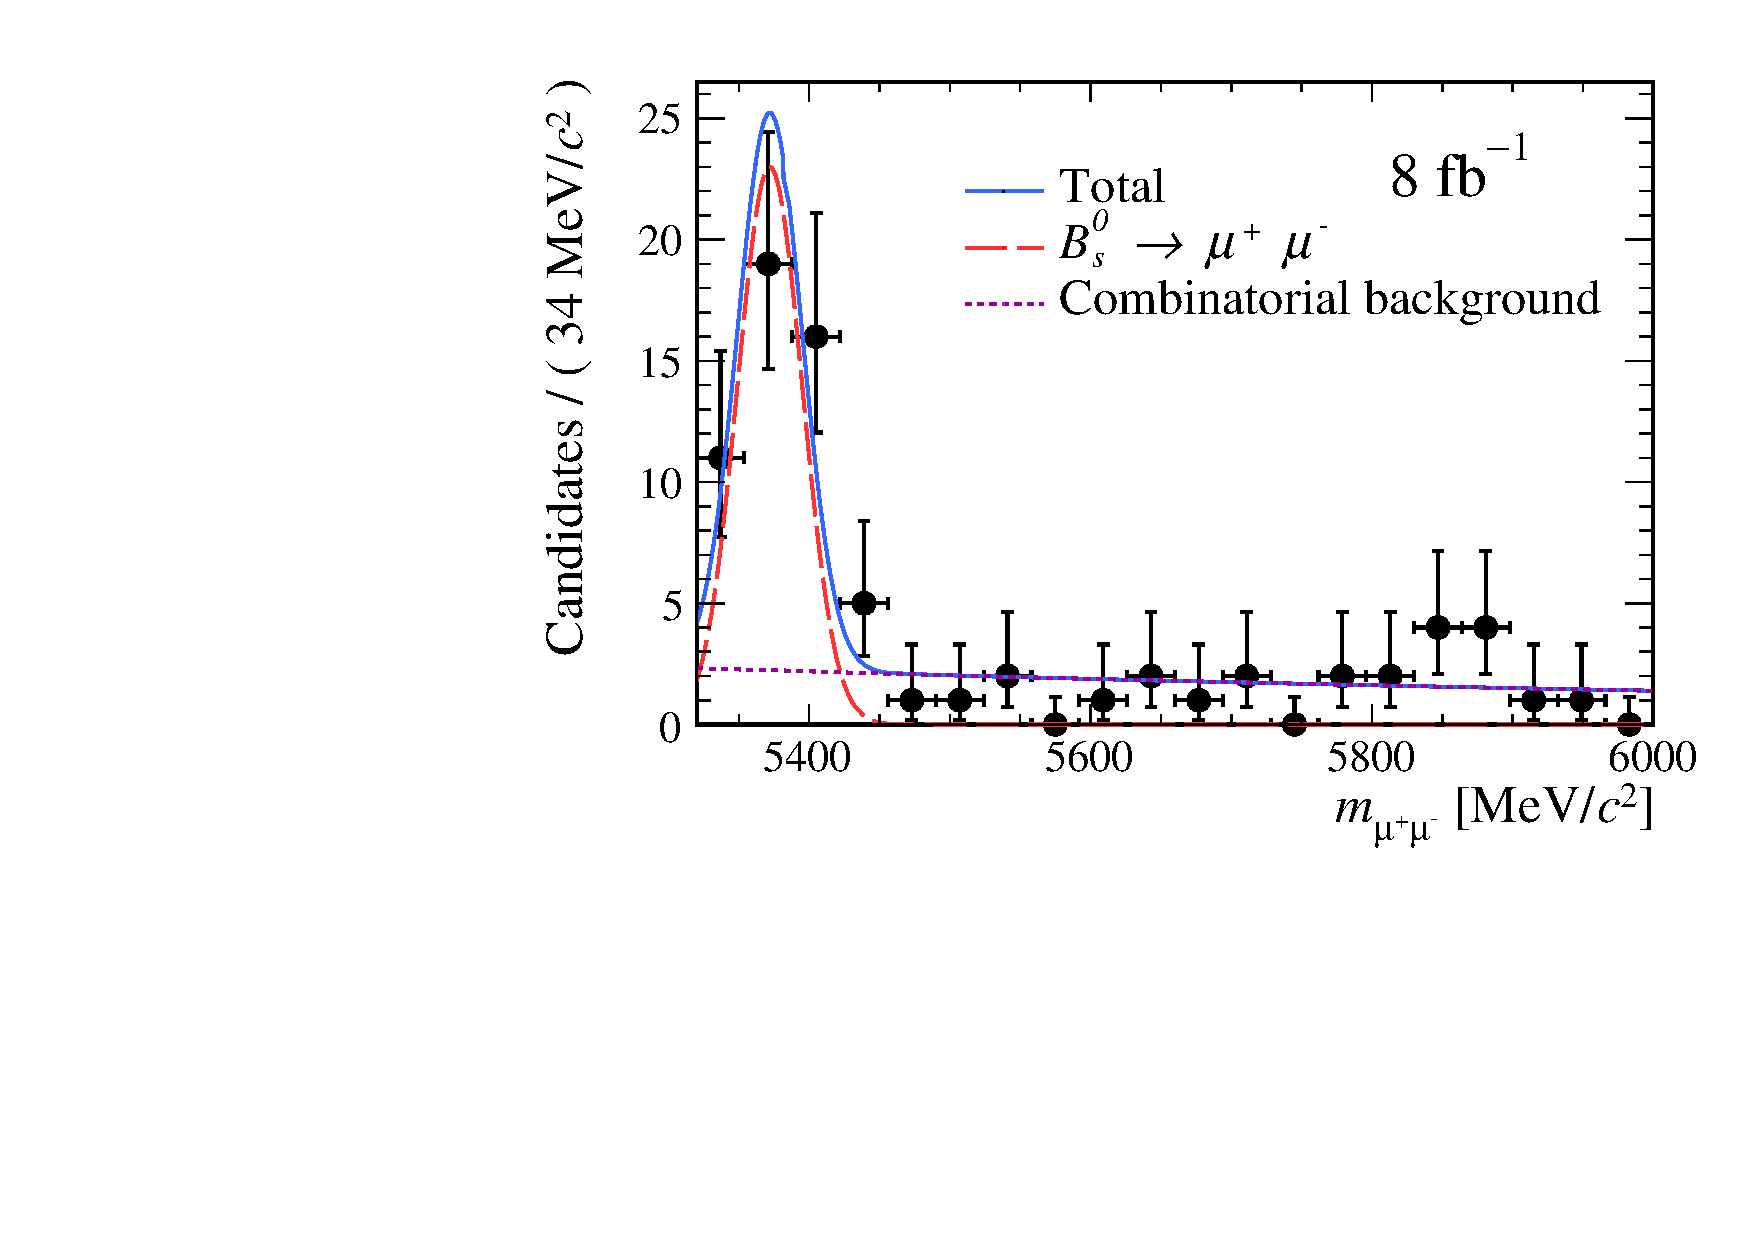
\includegraphics[width=0.49\textwidth]{./Figs/Summary/8fb_mass.pdf}
        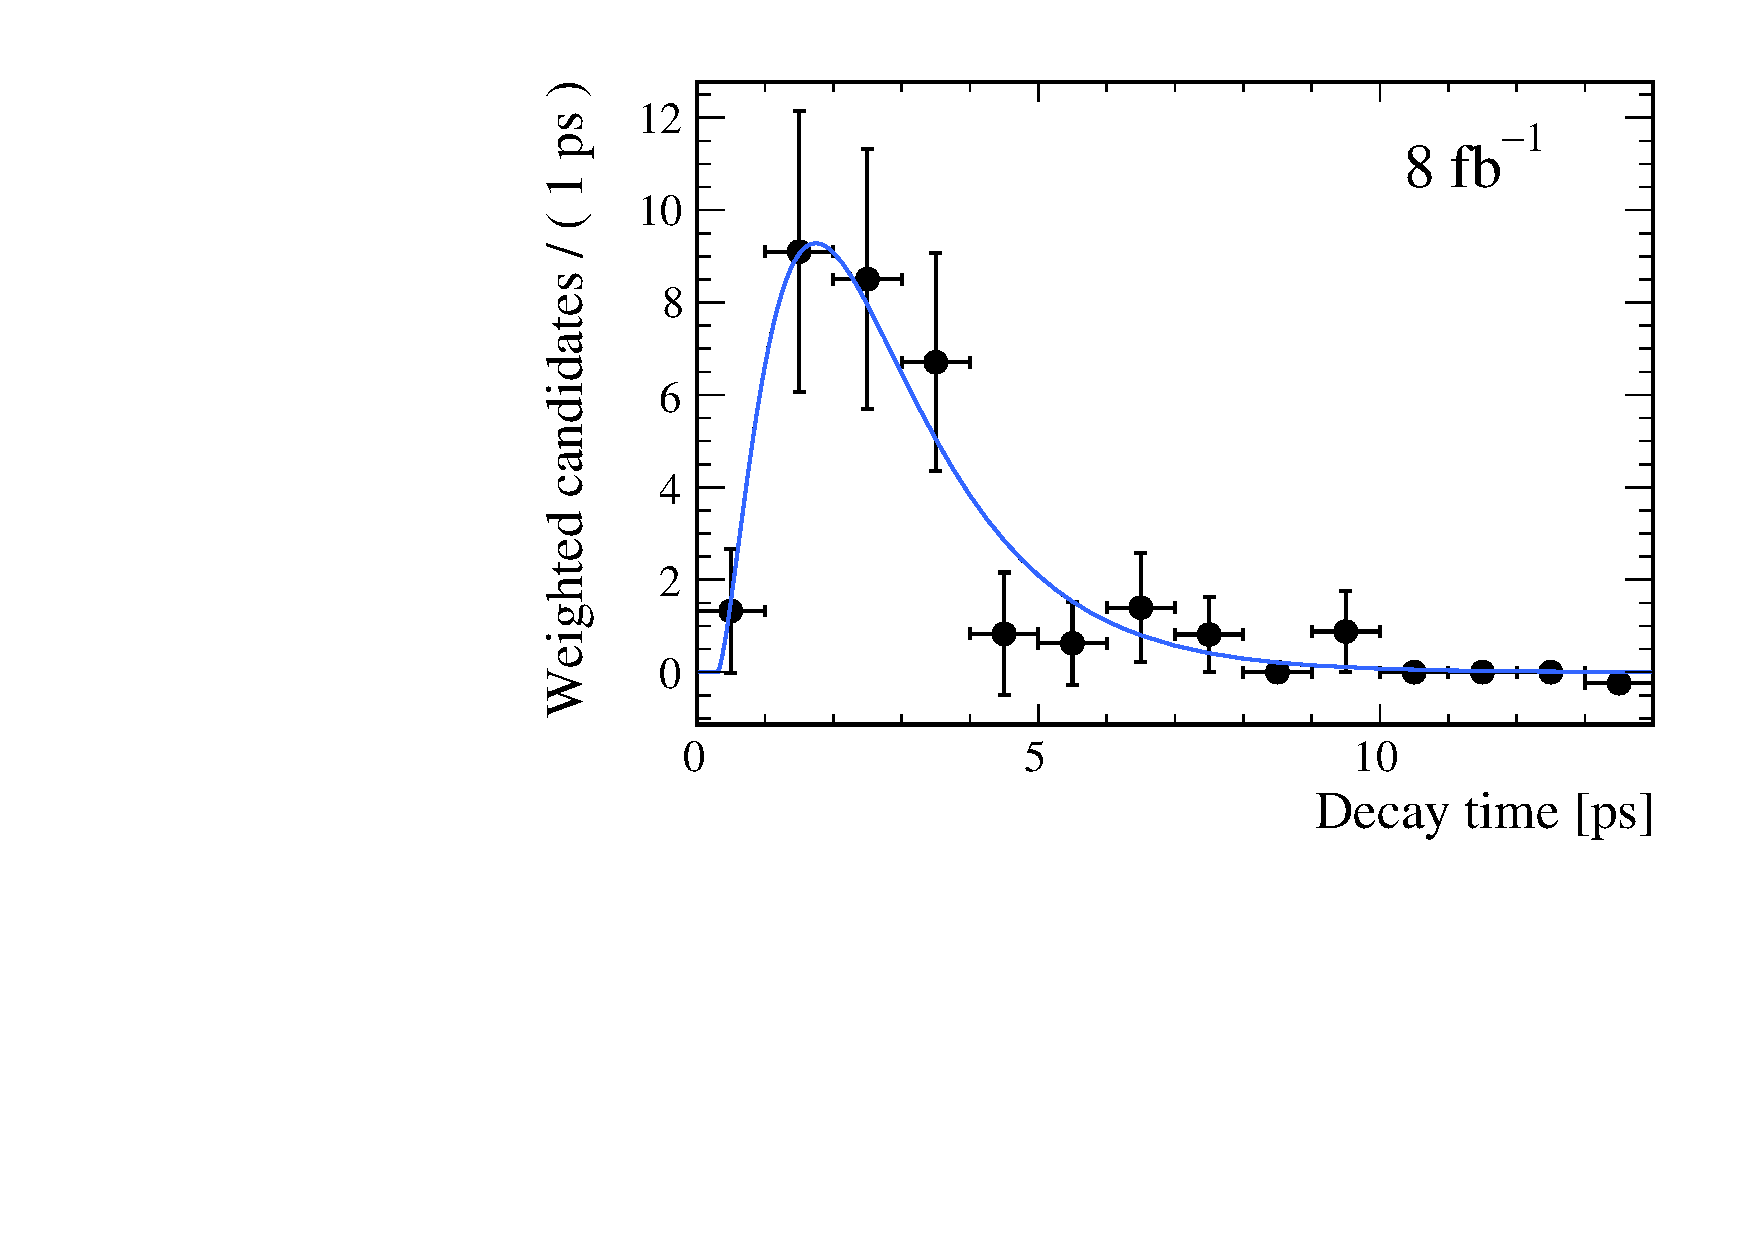
\includegraphics[width=0.49\textwidth]{./Figs/Summary/8fb_time.pdf}
        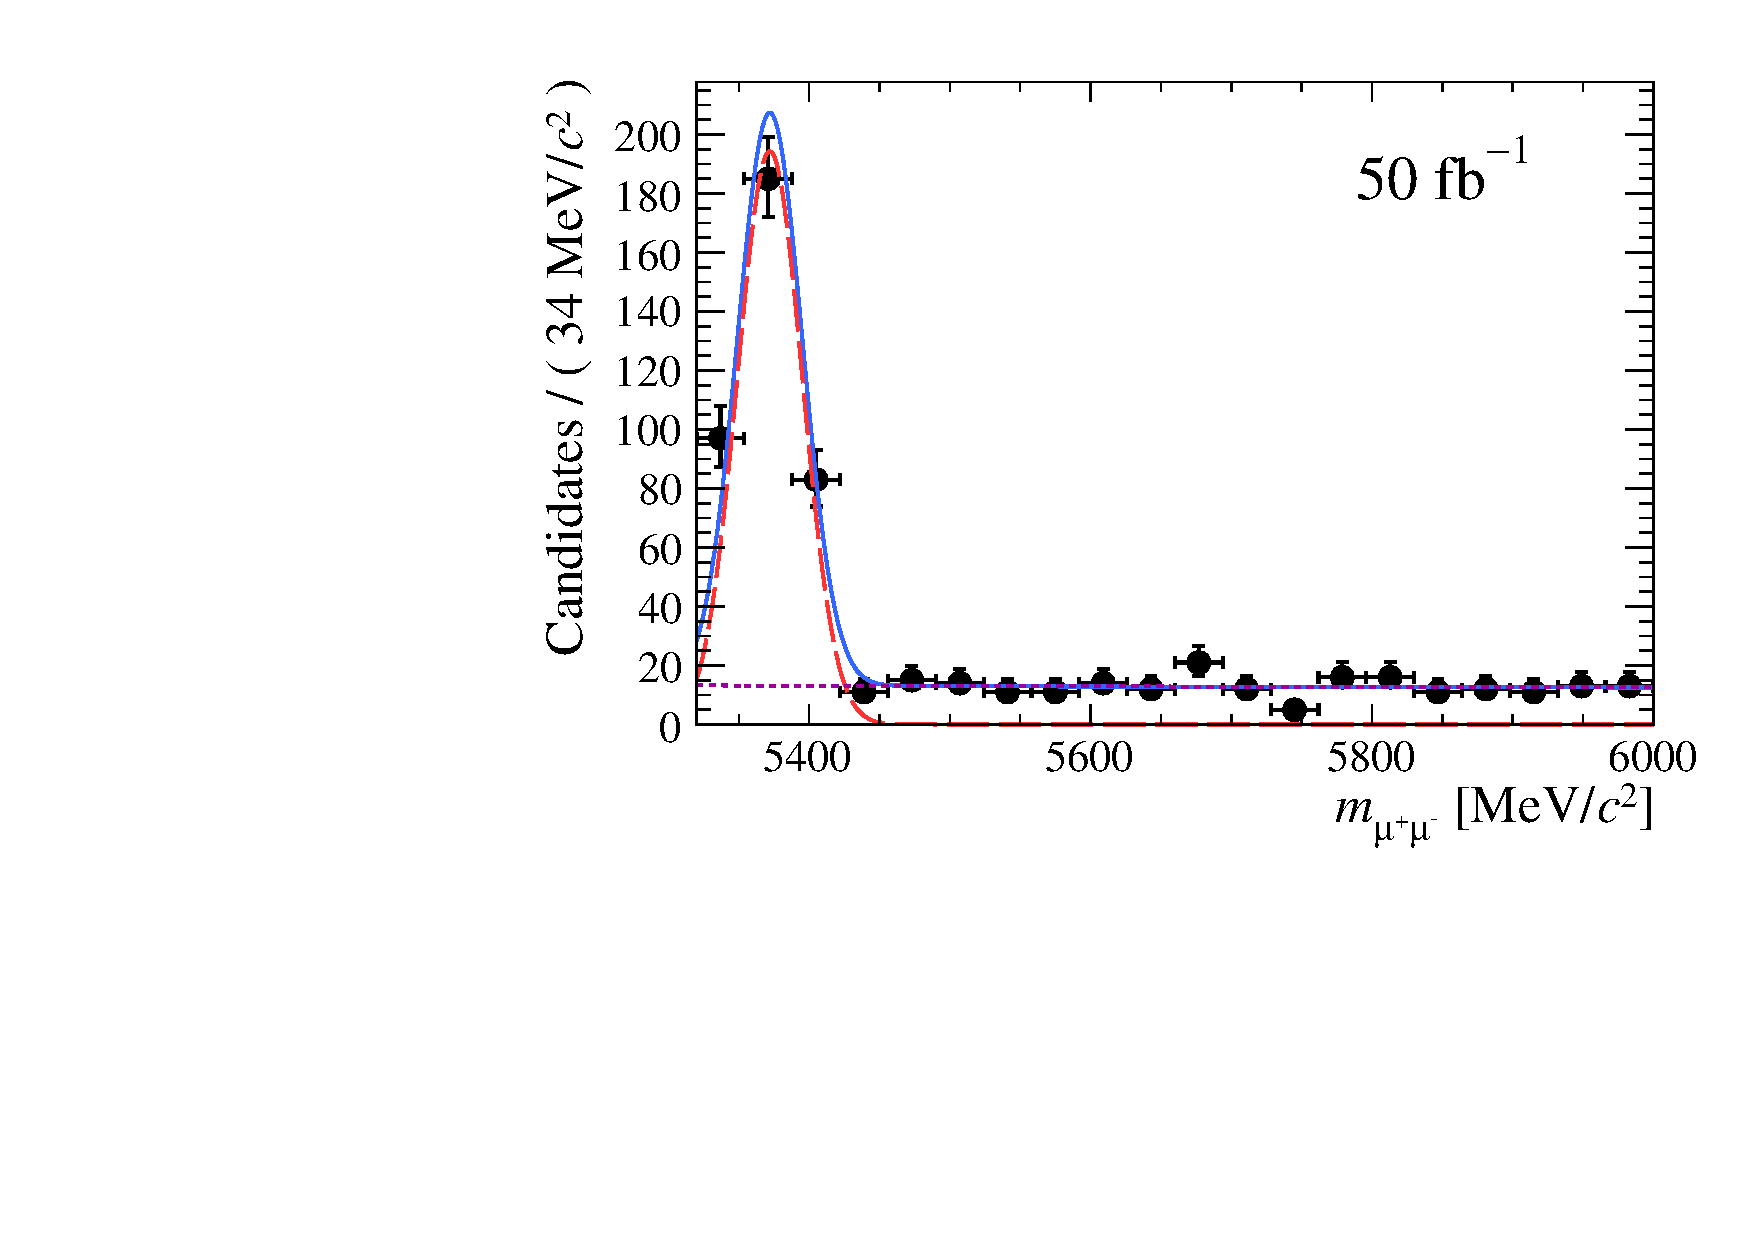
\includegraphics[width=0.49\textwidth]{./Figs/Summary/50fb_mass.pdf}
        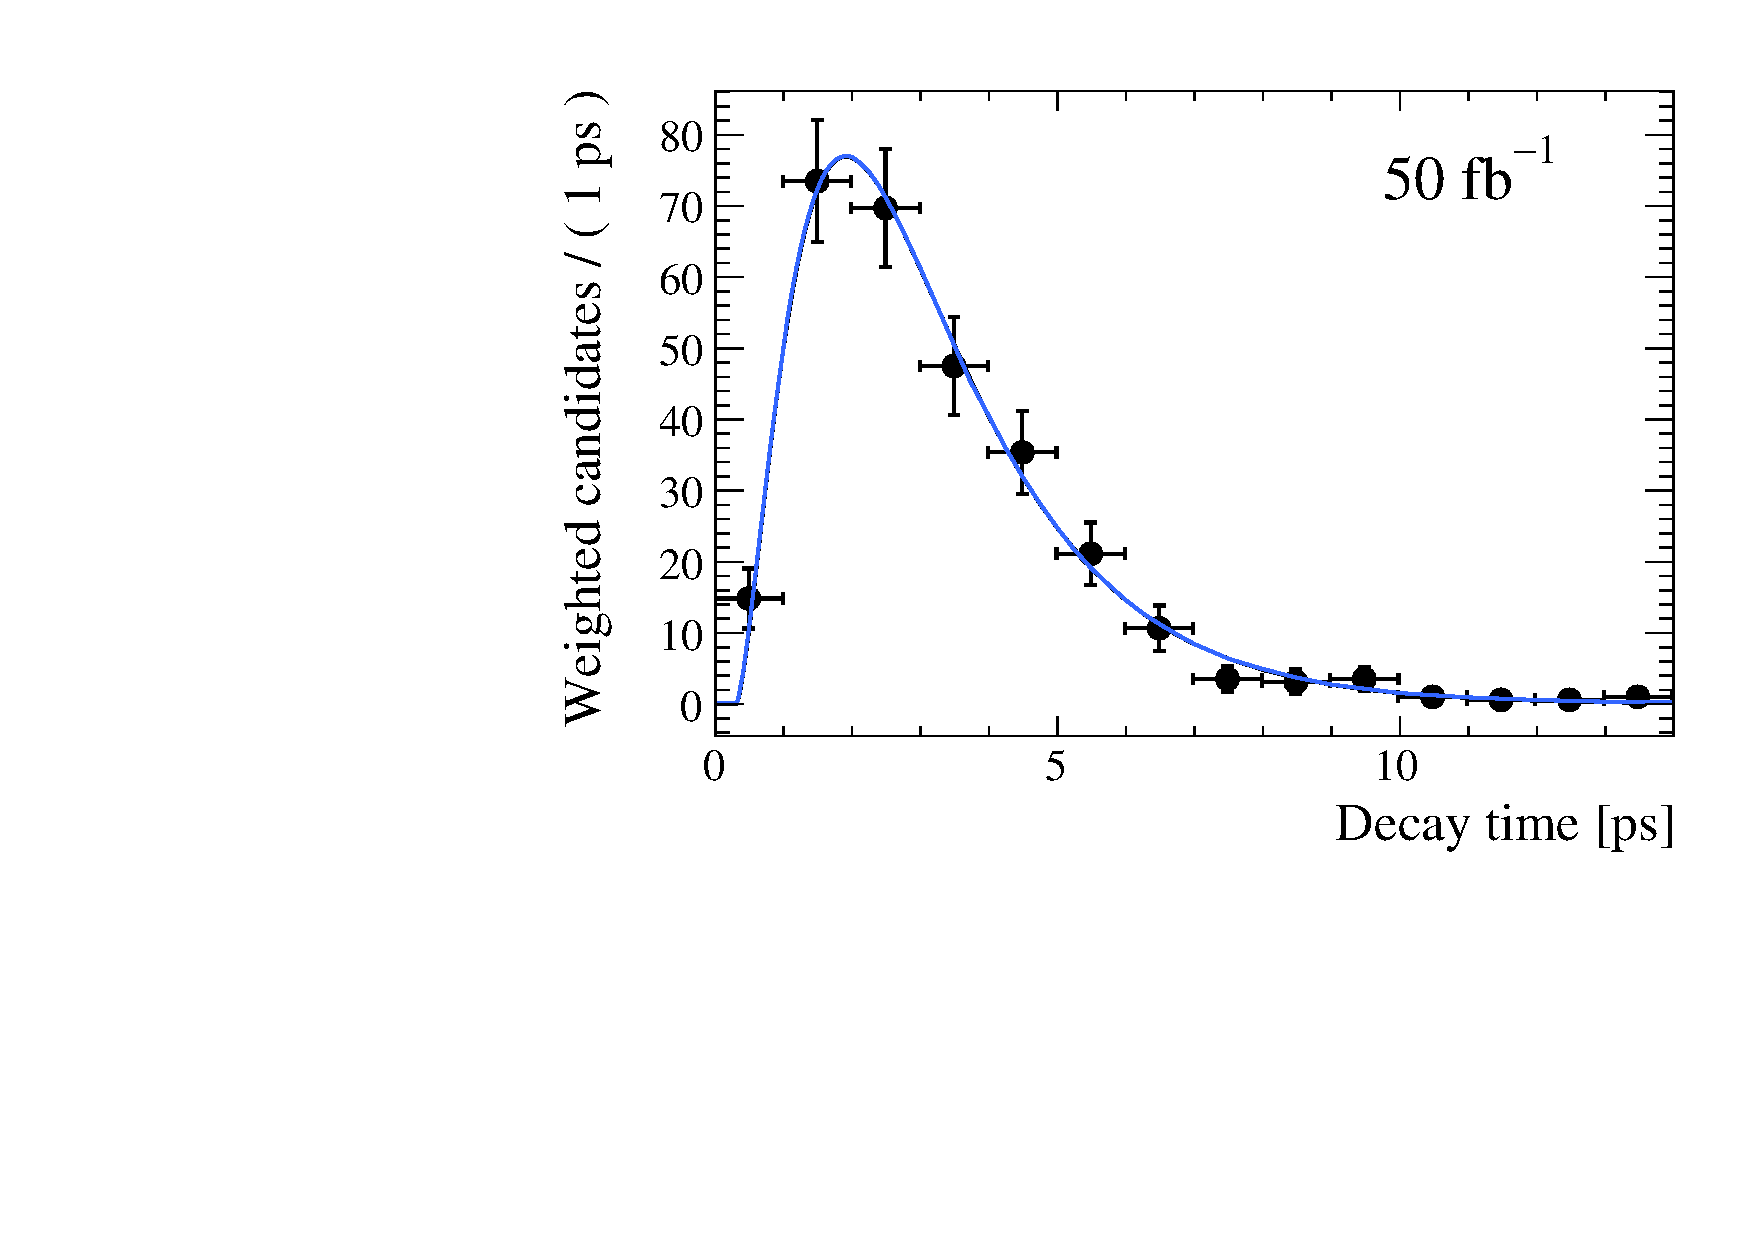
\includegraphics[width=0.49\textwidth]{./Figs/Summary/50fb_time.pdf}
        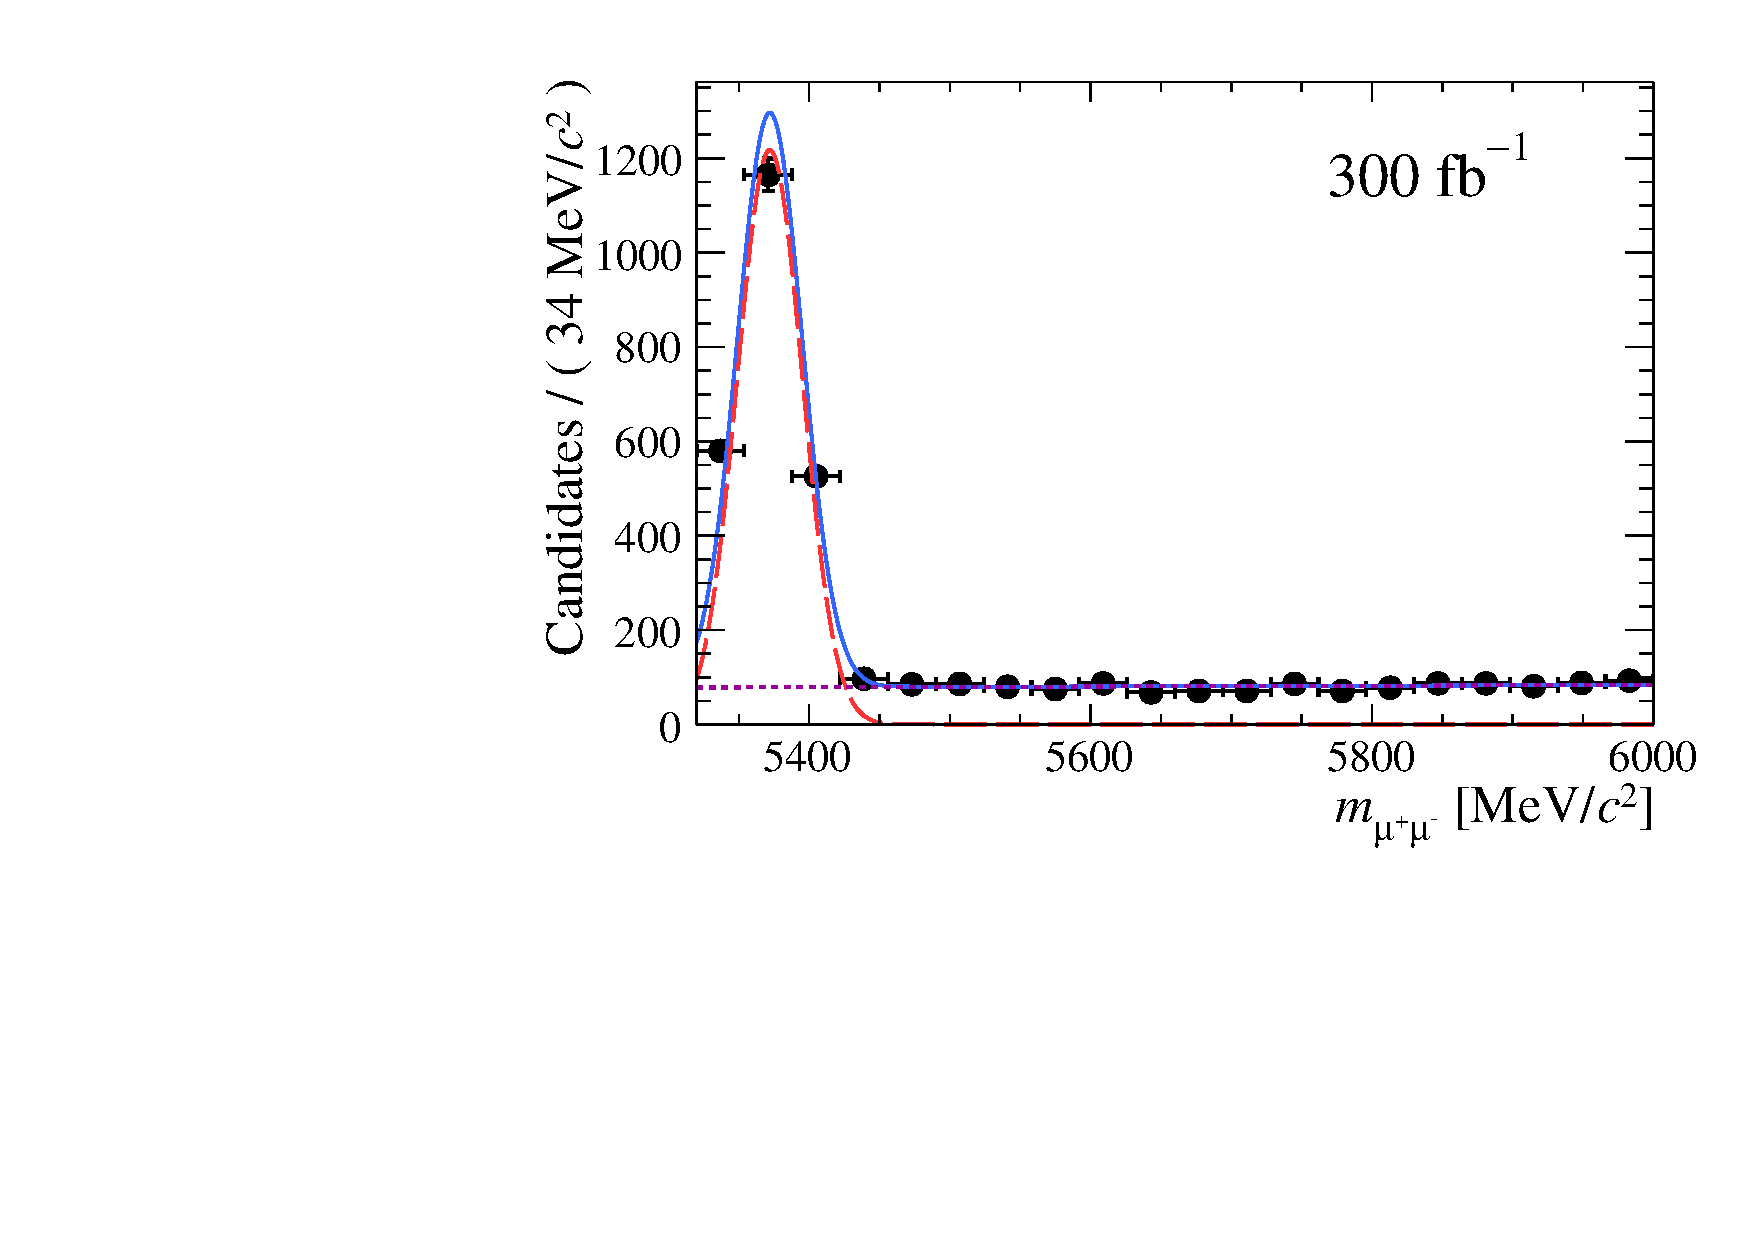
\includegraphics[width=0.49\textwidth]{./Figs/Summary/300fb_mass.pdf}
        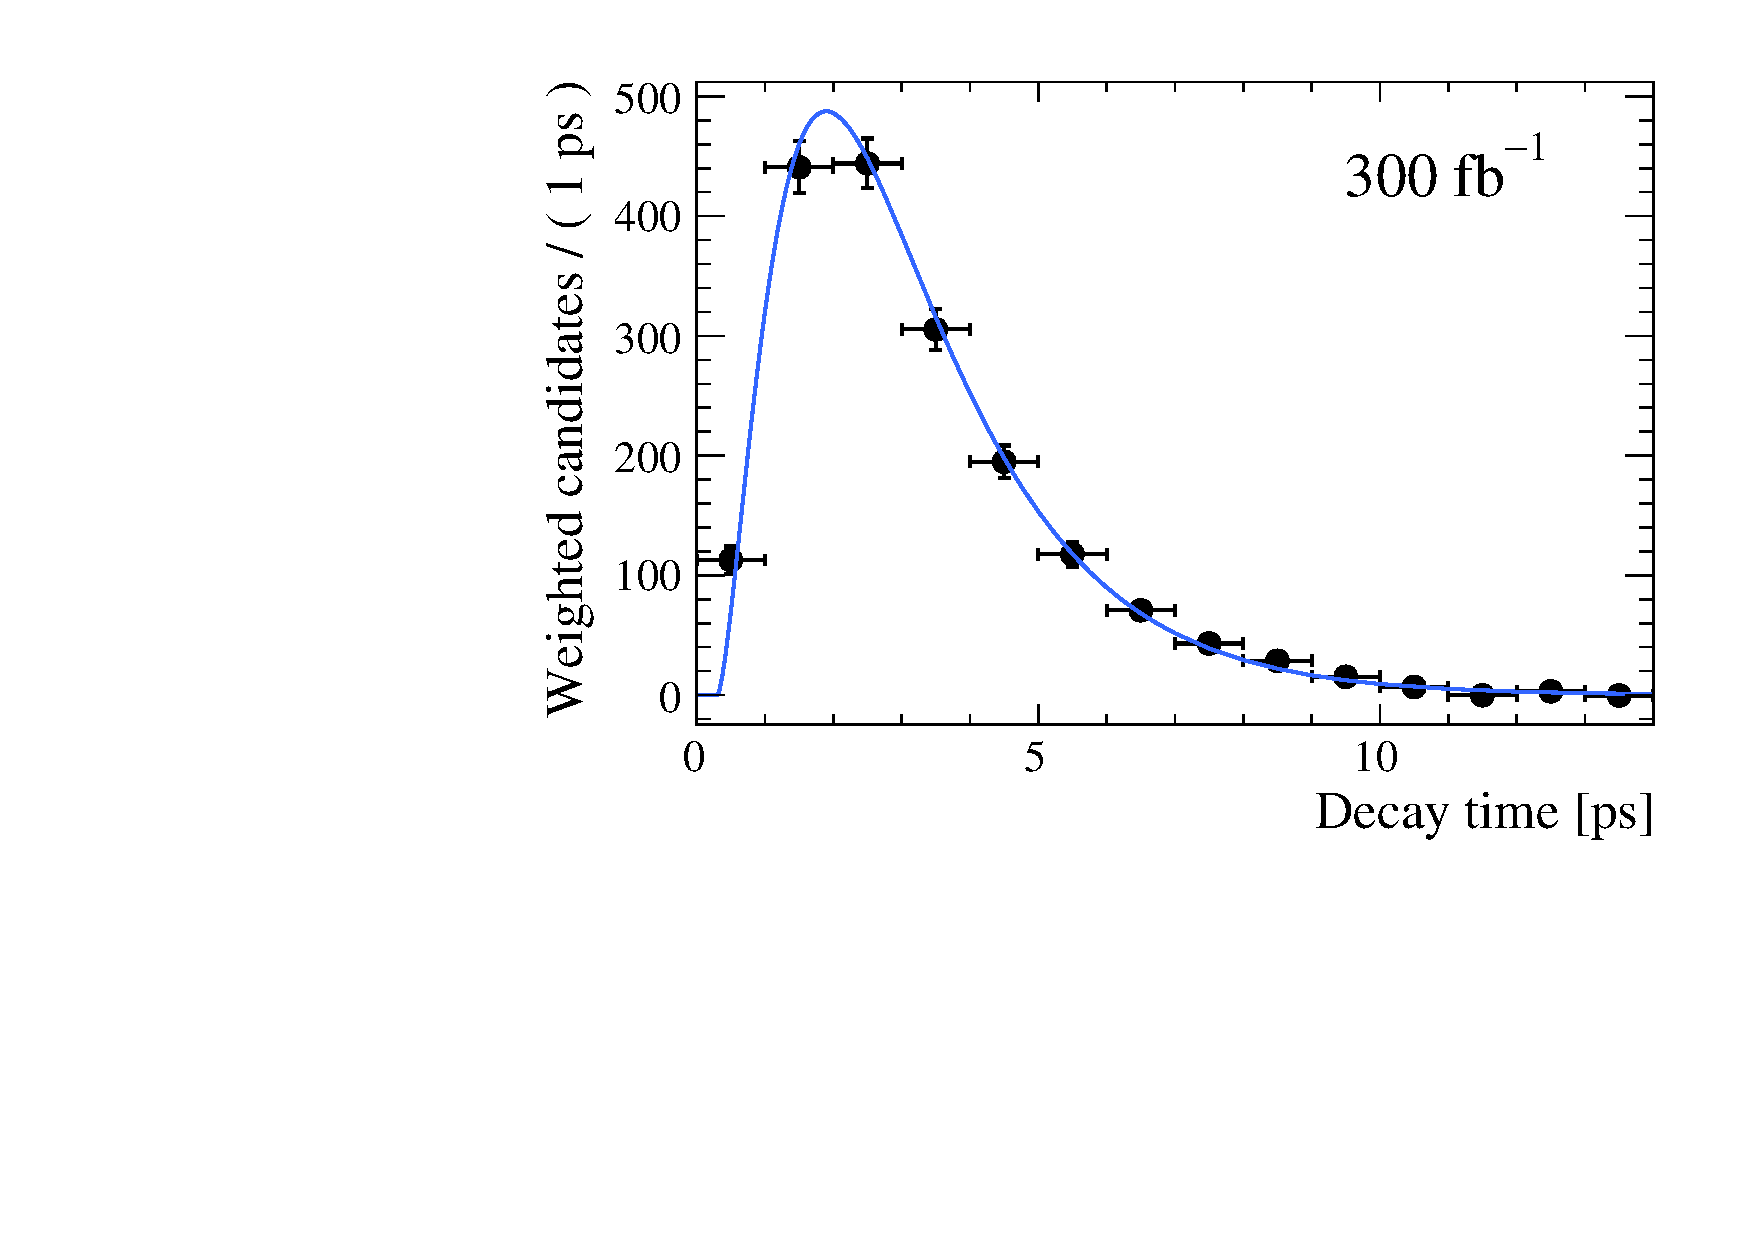
\includegraphics[width=0.49\textwidth]{./Figs/Summary/300fb_time.pdf}
    \caption{The expected mass and decay time distributions for \bsmumu candidates to measure the \el with 8, 50 and 300~\fb determined from the observed number of \bsmumu and combinatorial background decays in 4.4~\fb of Run~1 and Run~2 data, the expected number f mis-identified background and \bdmumu decays and assuming the SM \bsmumu \BF.}
    \label{fig:expected_dist}
\end{figure}





The current systematic uncertainty is 0.05 \ps which is too large to allow possible NP effects to be observed. However, several components contributing to the total, such as the fit accuracy and the acceptance function systematic, will be reduced with the availability of more data enabling greater precision on the measurement. With more data, an alternative analysis approach could be used which would reduce the systematic uncertainties on the \el, the selection criteria can be designed so that it does not bias \bsmumu decay time distribution, therefore removing the need for an acceptance function and the associated systematic.
%Do I want to include more discussion on this?? Or prehaps add as a appendix? I don't think a long discussion will add much here but prehaps the details could be useful or someone will ask about it ....


The study of \bmumu decays has been in progress for over 30 years and with the energy and luminosity available at the LHC, the study of these decays is just as interesting as it ever was. As more data is collected by the LHCb experiment NP effects will have less and less space to hide, it will either be seen in \bmumu decays or these decays will place ever tighter constraints on BSM theories. 
